\documentclass[a4paper]{article}
\usepackage[utf8]{inputenc}
\usepackage[english]{babel}
\usepackage{amsmath} % per ambienti tipo cases
\usepackage{amssymb}
\usepackage{mathtools}
\usepackage{siunitx}
\usepackage{graphicx} % per includere figure
%\usepackage{subfigure}
\usepackage{booktabs} % per le tabelle
\usepackage{caption}
\usepackage{fancyhdr}
\usepackage{hyperref}
\usepackage[section]{placeins}
\usepackage{microtype}
\usepackage{caption}
\usepackage{subcaption}
\captionsetup[subfigure]{labelfont=rm}
\usepackage{verbatim} %multiline comments
%\usepackage[backend=biber, style=numeric, safeinputenc, sorting=none]{biblatex}
%\addbibresource{source.bib}	% uncomment for bibliography



%opening
\title{}
\author{}

\pagestyle{fancy}
\lhead{Musical Acoustics}
\chead{HL2}
\rhead{10743504, 10751919}
\newcommand{\Rarrow}{\mbox{\Large$\Rightarrow$}}

\begin{document}

\begin{titlepage}	
	\newcommand{\HRule}{\rule{\linewidth}{0.5mm}} % Defines a new command for horizontal lines, change thickness here
	
	\center % Centre everything on the page
	
	%------------------------------------------------
	%	Headings
	%------------------------------------------------
	
	
\includegraphics[width=.4\textwidth]{Logo_Politecnico_Milano.png}\\[0.4cm]
	\textsc{\LARGE}\\[0.3cm] % Main heading such as the name of your university/college
	
	\textsc{\large MSc. Music and Acoustic Engineering}\\[1cm] % Minor heading such as course title
	
	\textsc{\Large Musical Acoustics - A.Y. 2020/2021}\\[0.5cm] % Major heading such as course name
	
	%------------------------------------------------
	%	Title
	%------------------------------------------------
	
	\HRule\\[0.4cm]
	
	{\huge\bfseries HL2 – Electric Analogs}\\[0.4cm] % Title of your document
	
	\HRule\\[1.5cm]
	
	
	
	{\large\textit{Authors' IDs:}}\\
	10743504, 10751919, % Your name
	%\\ \textsc{Gruppo 11}
	
	%------------------------------------------------
	%	Date
	%------------------------------------------------
	
	\vfill\vfill\vfill % Position the date 3/4 down the remaining page
	
	{\large\today} % Date, change the \today to a set date if you want to be precise
	
	%------------------------------------------------
	%	Logo
	%------------------------------------------------
	
	\vfill\vfill
	%\includegraphics[width=0.2\textwidth]{Politecnico_di_Milano.eps}\\[1cm] % Include a department/university logo - this will require the graphicx package
	
	%----------------------------------------------------------------------------------------
	
	\vfill % Push the date up 1/4 of the remaining page
	
	
\end{titlepage}

\section{Simulating a Helmholtz resonator}

\begin{figure}[h!]
	\centering
	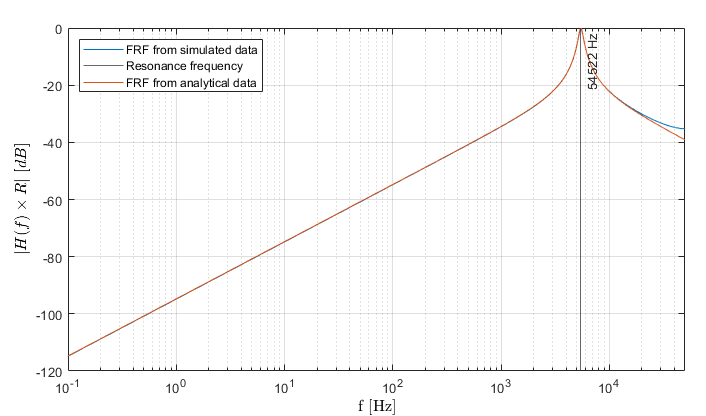
\includegraphics[width=0.7\linewidth]{es1.png}
	\caption{Plot of the magnitude $R|H(f)|$ in dB, both for the analytical expression and for the Simscape simulation. The resonance frequency is also highlighted.}
	\label{fig:es1}
\end{figure}

The Helmholtz resonator can be modelled in the impedance analogy as an RLC series circuit, with:

\begin{align*}
	R &= \frac{\rho c}{S}\, &
	L &= \frac{\rho l}{S}\, &
	C &= \frac{V}{\rho c^2}
\end{align*}

This model has been implemented in Simscape, and it can be seen in \texttt{Es1.slx}. In order to obtain the frequency response of the system we are interested in retrieving the current signal (which in our analogy represents the volume flow $U$) from the simulation: this can be done by simply adding an amperometer in the loop, in series with the other components.

Moreover, we will need to provide a known input to the system, and specifically an impulsive one, since the FRF is the Fourier transform of the impulse response. We can create an input signal in Simulink by subtracting together two discrete step functions that are offset by 1 sample with eachother, obtaining a discrete impulse. The Simulink signal is then converted into a Simscape physical signal and fed to a controlled voltage source block that will serve as the generator for our circuit. Thus, the input voltage (i. e. pressure) signal and the resulting current can be sent to a \texttt{To Workspace} Simulink block\footnote{The output of the amperometer will need to be converted into a Simulink signal first.} that will allow us to access the results with Matlab. The FRF can then be computed as the ratio between the volume flow and the input pressure (in the frequency domain):
$$ H(\omega) = \frac{U(\omega)}{p(\omega)} = \biggl( \mathrm{j}\omega L + R + \frac{1}{\mathrm{j}\omega C} \biggr)^{-1}$$
where the last member is the analytical expression of $H$ which is easily computed as the input admittance of the series of the three components.

The simulation has been carried out over 10 seconds, with a sampling frequency of 100 kHz. The frequency spectra of the resulting signals have been obtained by computing their DFT with Matlab's \texttt{fft} function. The result of the simulation is compared with the analytical expression for $H$ in Fig. \ref{fig:es1}, showing that the two are remarkably close up to the highest frequencies.




\section{The Helmholtz resonator tree}

By cascading several Helmoltz resonators in the manner shown in Fig. \ref{fig:tree}, we obtain what we refer to as a Helmholtz resonator tree. A tree of this kind is characterized by the parameters $N, K \in \mathbb{N}$, where $N$ is the height of the tree and $K$ is the branch division.

To realize different trees of this kind in Simscape, we set up a template of a subsystem containing a single Helmholtz resonator, as seen in Fig. \ref{fig:sims}, in order to keep things as tidy as possible. The Simscape models can be seen in the files named \texttt{RTNK.slx}, with $(N, K) = (1,2), (2,1), (2, 2), (2, 3), (3,2), (3,3)$.

\begin{figure}[h!]
	\centering
	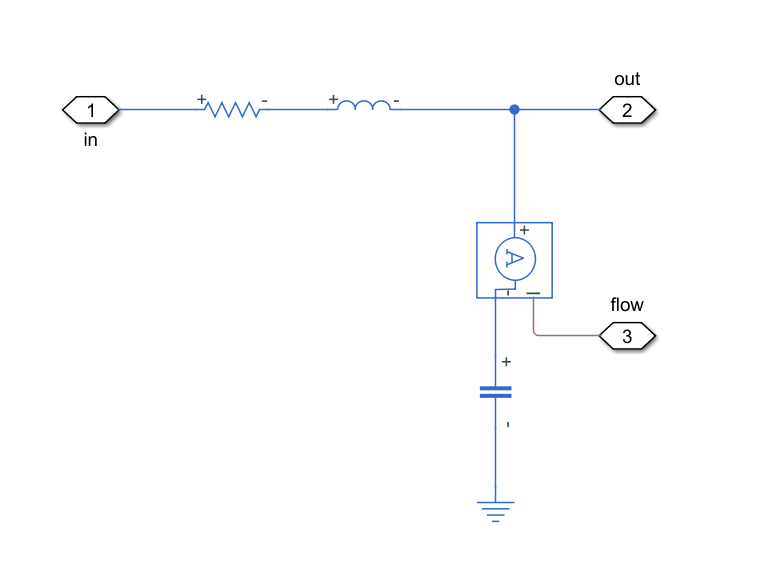
\includegraphics[width=0.7\linewidth]{sims.png}
	\caption{Single Helmholtz resonator subsystem in Simscape. The ports are points that can be accessed from outside the subsystem: ports 1 and 2 allow connections of the resonators with eachother and/or with the generator, while port 3 allows to read the value of the current flowing in the single loop.}
	\label{fig:sims}
\end{figure}

We computed a frequency response by reading the current at one of the resonators in the lowest level of the tree (the farthest from the tree inlet). Fig. \ref{fig:es2} shows the plots of the responses. We can see how incrementing the height of the tree seems to add a peak to the response, and indeed there seem to always be $N+1$ resonances. Conversely, increasing $K$ leaves the number of resonances unchanged, but the separation between neighboring peaks grows.



\begin{figure}[h!]
	\centering
	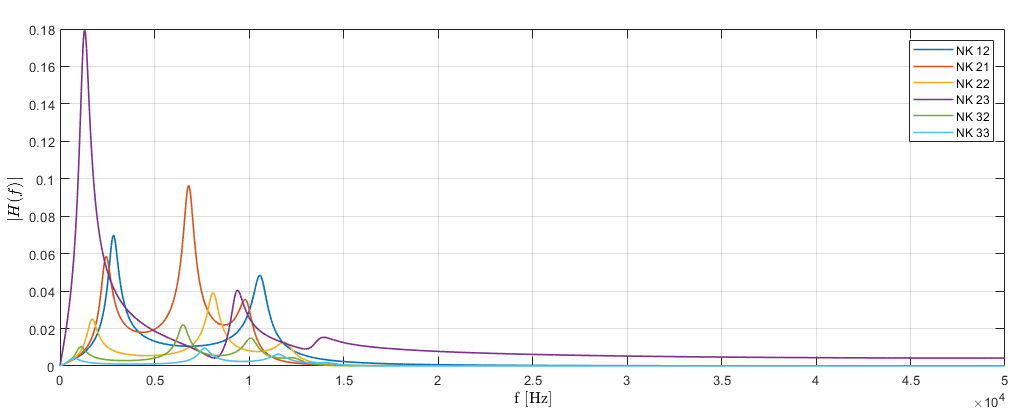
\includegraphics[width=0.7\linewidth]{es2.png}
	\caption{FRFs of the different trees at the bottom level.}
	\label{fig:es2}
\end{figure}



\end{document}